\documentclass[11pt]{article}
%Gummi|065|=)
\usepackage{graphicx}
\usepackage[utf8]{inputenc}
\usepackage[russian]{babel}
\title{\textbf{Прогнозирование курсов криптовалют}}

\begin{document}

\maketitle

\section{Обработка предоставленного датасета}
Предоставленный датасет представляет из себя 5 видов данных - с промежутками в день, час, 30 мин, 5 мин, 1 мин. Для каждого промежутка есть данные для многих валютных пар. 

Первое, что мы захотели сделать - составить для каждого промежутка датасет охватывающий период времени, являющийся пересечением доступных периодов времени для всех валютных пар. То есть такой период времени, для которого известны все валютные пары. Но, к сожалению, выяснилось, что это пересечение равно 0. Конечно можно взять просто все данные, но тогда на краях будет уж очень много пропусков, и скорее всего это будет плохо. (В качестве эксперимента мы так и сделали второй опцией). Поэтому мы провели следующий анализ данных - для каждого k от 1 до количества валютных пар мы нашли максимальное по размеру пересечение хотя бы k валютных пар. График этой величины от k для датасета oneMin представлен на рис \ref{fig:oneMin_intersections}
\begin{figure}[!htb]
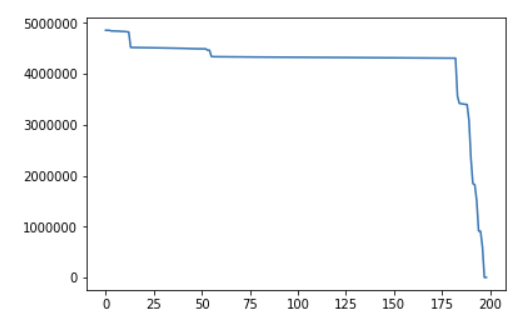
\includegraphics[width = 15cm]{oneMin_intersections.png}
\caption{oneMinintersections}
\label{fig:oneMin_intersections}
\end{figure}

Имеем, что для k = 1 можно взять довольной большой отрезок времени равный собственно максимальному периоду, для которого известен курс какой-либо валютной пары. Для k близкого к суммарному количеству валютных пар (примерно  200) период времени, для которого известны одновременно какие-то k валютных пар уже довольно мал. Для k равного количеству валютных пар этот период равен 0. 

Для датасетов oneMin, fiveMin, thirtyMin, hour этот график примерно похож на \ref{fig:oneMin_intersections}. И для них очень разумно сделать отсечение, показанное на рис \ref{fig:chosen}. 
\begin{figure}[!htb]
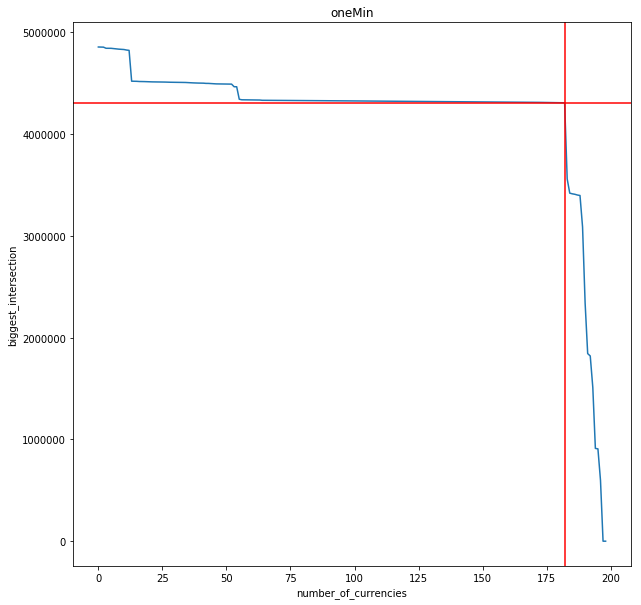
\includegraphics[width = 15cm]{chosen.png}
\caption{chosen}
\label{fig:chosen}
\end{figure} 

Таким образом мы одновременно сохраняем почти все валютные пары, и почти весь временной период.

Для дневного датасета график выглядит по-другому (\ref{fig:days})
\begin{figure}[!htb]
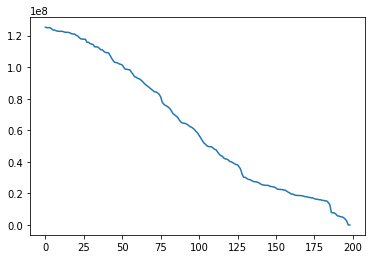
\includegraphics[width = 15cm]{days.png}
\caption{days}
\label{fig:days}
\end{figure} 

Для него мы решили вообще не делать никакой обрезки.

Итого имеем 9 датасетов - по 2 для oneMin, fiveMin, thirtyMin, hour - один полный, который охватывает весь промежуток времени и все валютные пары, но в нем очень много пропусков, особенно по краям,  и другой, который охватывает почти весь промежуток времени, и почти все валютные пары, пропусков в котором не так много, и которые обусловленны только внутренними пропусками для валютных пар, а не несоответствием их временных периодов.

И для дневного датасета только полный.

Подробнее об этой процедуре можно посмотреть в тетрадке "analyzing dataset.py"

\section{Сбор и обработка данных с hitbtc}
Мы собрали данные для 21 валютной пары с шагом примерно в секунду для 44 с половиной дней. 

Выглядит это примерно так: (рис \ref{fig:ETH_BTC_hitbtc})
 
\begin{figure}[!htb]
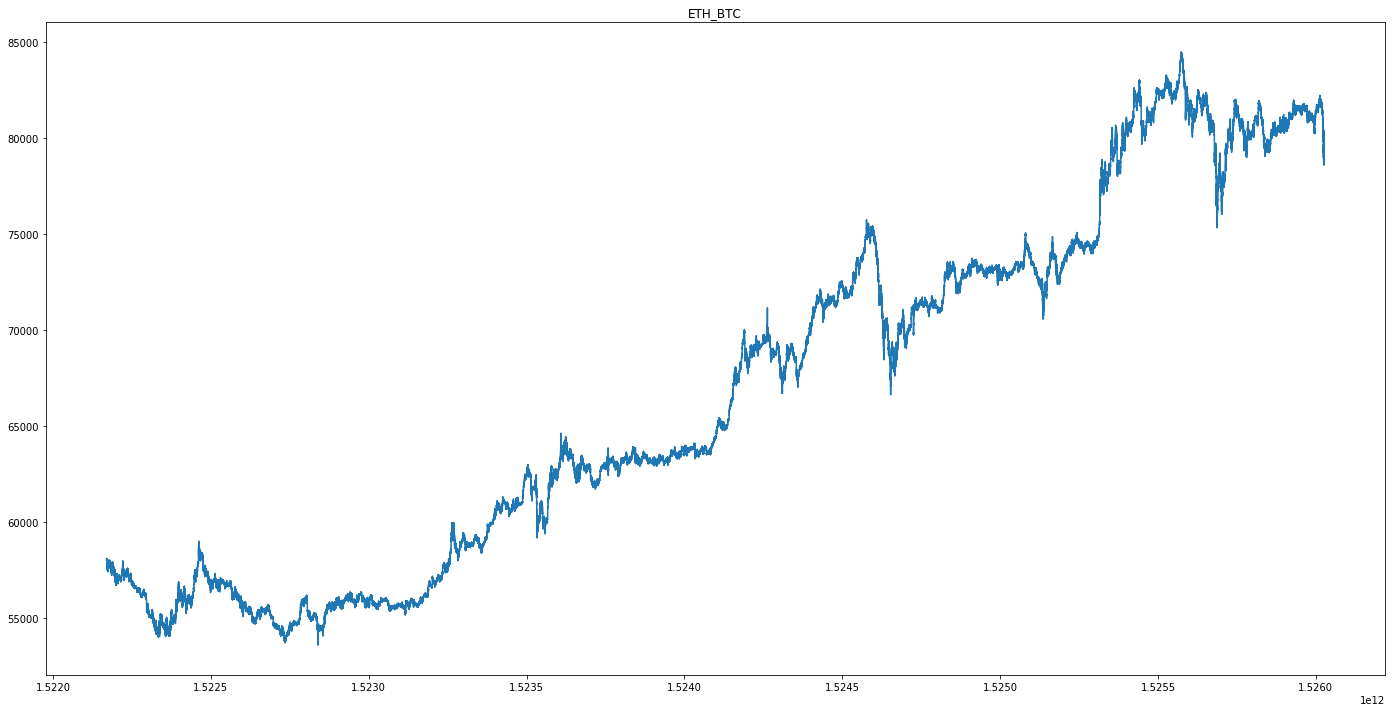
\includegraphics[width = 15cm]{ETH_BTC_hitbtc.png}
\caption{hitbtc}
\label{fig:ETH_BTC_hitbtc}
\end{figure} 

И все вроде бы ровно, но 1) для каждой валютной пары есть свой timestamp - то есть данные имеют вид не какой-то timestamp и значения всех валютных пар для него, а имеет вид троек - для каждой валютной пары свой timestamp, и ask и bid в этот момент. 2) timestamp-ы идут не идеально раз в секунду а с некоторой погрешностью. 3) в данных случаются довольно большие пропуски. А именно если построить график значения  timestamp-а от его порядкового номера в датасете, то получится следующее (\ref{fig:timestamp_hitbtc})

\begin{figure}[!htb]
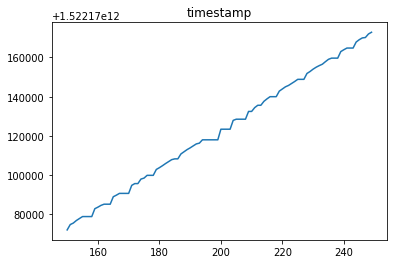
\includegraphics[width = 15cm]{timestamp_hitbtc.png}
\caption{timestamps}
\label{fig:timestamp_hitbtc}
\end{figure} 

То есть имеются довольно сильные залипания иногда продолжительностью до 20 секунд. 

Чтобы привести эти данные к нормальному виду было решено использовать следующий алгоритм - выбирается общая сетка из таймстемпов с шагом dT. Далее для очередного значения этого общего timestamp-а для каждой валютной пары смотрится - есть ли известные значения для этой пары около этого timestamp-а с обоих сторон на расстоянии не более чем delta. Если есть то значения курса в этом значении timestamp-а выбирается равным линейной интерполяции значении курсов слева и справа. Если нет, то ставится пропуск.

Таким образом мы сгенерировали 2 датасета - для первого dT = 100 сек, delta = 5 сек, для второго dT = 3600 сек, delta = 50 сек. 

В качестве значений курсов в обоих случаях бралось среднее между аском и бидом. 

Подробнее об этой процедуре можно посмотреть в тетрадке aligning hitbtc timestamps

\section{Тесты на искусственных данных}
Мы реализовали метод, предложенный в статье и решили проверить его работоспособность на синтетических данных. А именно в данной модели данные имеют следующий вид - есть некоторое латентное пространство меньшей размерности, в котором данные почти подчиняются неким линейным рекурентным соотношениям, а данные в исходном пространстве являются линейной функцией от данных в латентном пространстве. По такой схеме и были сгенерированны синтетические данные - сначала в соответствии с рекурентными соотношениями были сгенерированы даные в латентном пространстве, далее была случайно сгенерирована матрица перехода в реальное пространство. 

Если генерить данные по линейным рекурентным соотношениям с абы-какими коэффициентами - то возможны 2 сценария - все собственные числа будут меньше 1 - тогда очень скоро последовательность выродится в 0, или если есть хотя бы 1 собственное число большее 1 - тогда последовательность скоро разойдется. Чтобы избежать этого были подобраны специальные коэффициенты этих рекурентных соотношений. А именно с собственными числами $1, \cos(\sqrt(2)) +- \sin(\sqrt(2)) * i$
(иррациональный период был выбран чтобы избежать периодичности). 

Так же было добавлено 2 типа шума - при генерации рекурентной последовательности в латентном пространстве и случайная прибавка к итоговому Y.

На этих данных наша библиотека сумела успешно восстановить матрицу W (коэффициенты рекурентной последовательности) с погрешностью около 0.01 и предсказать последовательность в будущее (\ref{fig:synthetic_low_noise})

\begin{figure}[!htb]
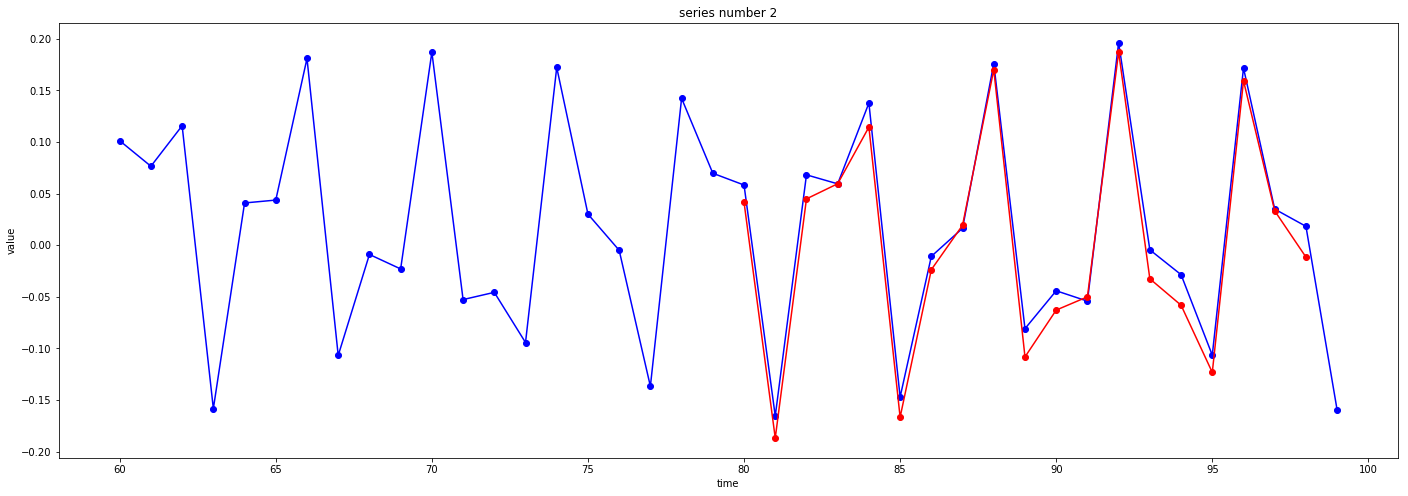
\includegraphics[width = 15cm]{synthetic_low_noise.png}
\caption{low noise}
\label{fig:synthetic_low_noise}
\end{figure} 


Так же был проведен эксперимент с существенно большим шумом (в 10 раз больше)
(\ref{fig:huge_noise}): 

\begin{figure}[!htb]
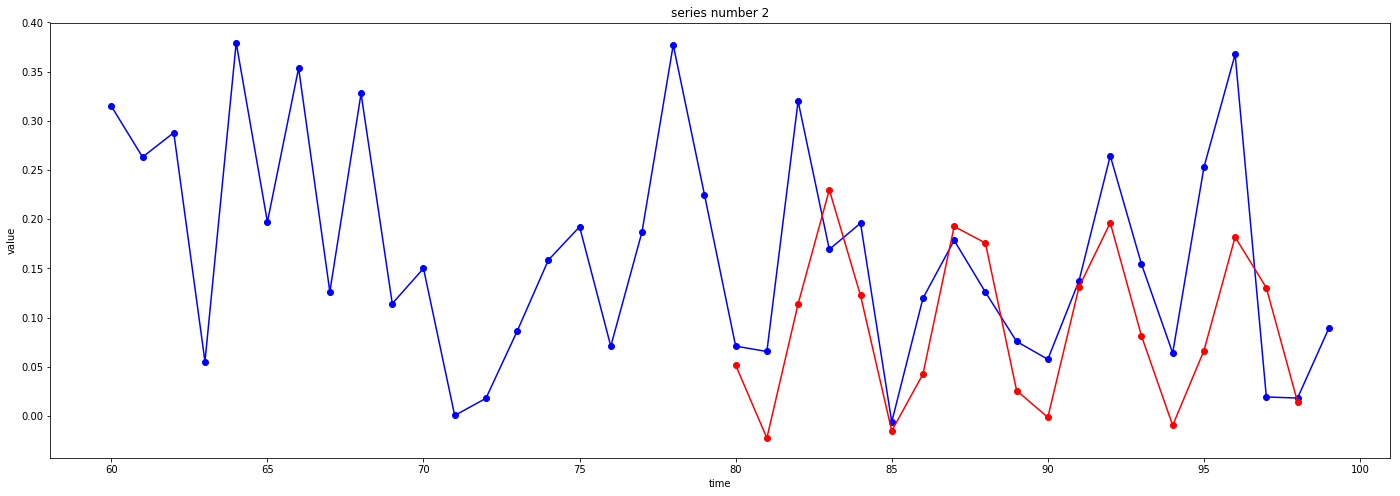
\includegraphics[width = 15cm]{huge_noise.png}
\caption{huge noise}
\label{fig:huge_noise}
\end{figure} 

А без шума (\ref{fig:no_noise}) предсказания почти идеальны

\begin{figure}[!htb]
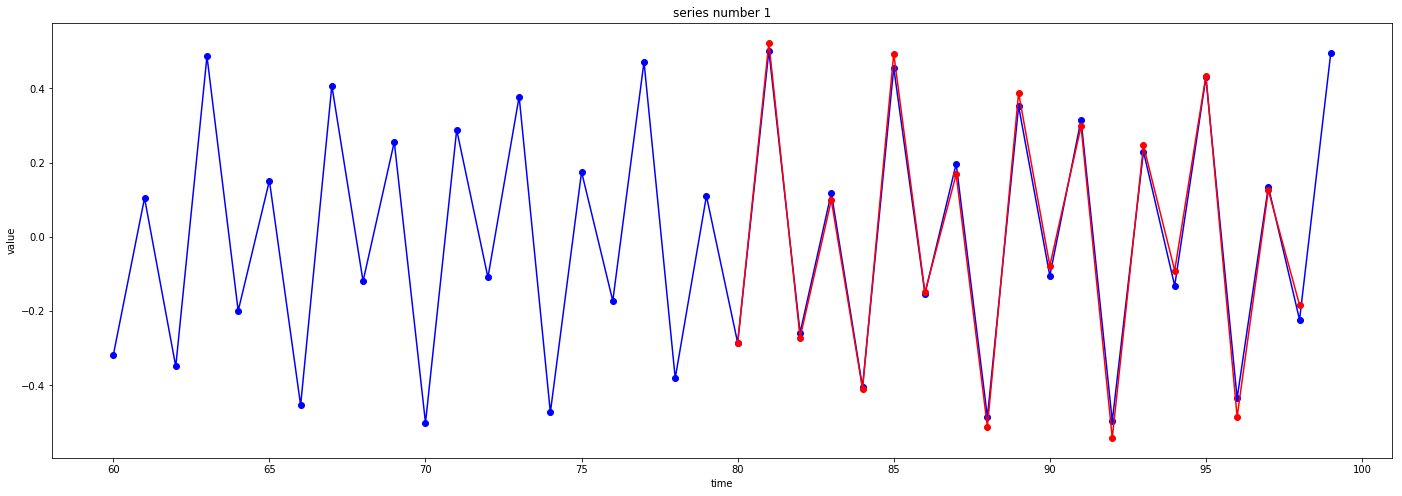
\includegraphics[width = 15cm]{no_noise.png}
\caption{no noise}
\label{fig:no_noise}
\end{figure} 

Так же эти эксперименты - это очень хороший тест на правильность нашей библиотеки.

Более подробно их можно изучить в тетрадке testing on synthetic data

\section{Временные замеры}
Далее мы решили измерить время работы нашей библиотеки и эмпирически измерить ассимптотики от разных величин. 
Для этих измерений был выбрал датасет c hitbtc, который побольше - с dT = 100 с. 

Итак 1) - время от итераций естественно растет линейно (\ref{fig:iteration_measurements}). 

\begin{figure}[!htb]
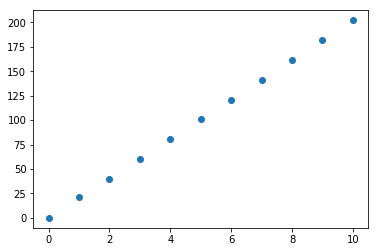
\includegraphics[width = 15cm]{iteration_measurements.png}
\caption{time dependence on number of iterations}
\label{fig:iteration_measurements}
\end{figure} 

Но тем не менее эта зависимость не точно прямо пропорциональная, потому что кроме итераций происходит еще некоторые операции, и поэтому далее время на итерации измерялось как время на 5 итераций минус время на 1 итерацию и делить на разницу в 4 итерации.

Зависимость времени от T тоже линейная, как и должно быть (\ref{fig:T_dependence}) 
\begin{figure}[!htb]
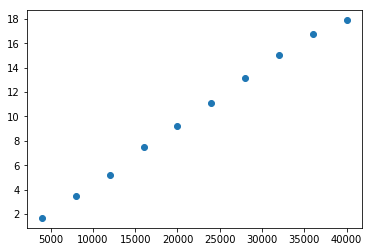
\includegraphics[width = 15cm]{T_dependence.png}
\caption{time dependence on T}
\label{fig:T_dependence}
\end{figure} 

Зависимость от размера множества лагом приведена на рис (\ref{fig:lags_size_dependence})
\begin{figure}[!htb]
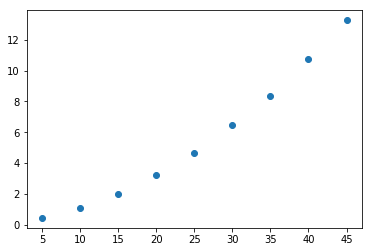
\includegraphics[width = 15cm]{lags_size_dependence.png}
\caption{time dependence on number of lags}
\label{fig:lags_size_dependence}
\end{figure} 

Она не линейная, и если вытащить показатель степени, зафитив прямую в логарифмическом масштабе, то получится примерно 1.6, при теоретическом 2.0. Но если зафитить прямую не на все данные, а на часть данных справа, то получится уже 1.8, что ближе к теоретическому значению. То есть отклонение происходит из-за наличия других членов асимптотики, чей относительный вклад тем больше, чем меньше измеряемый член. 

ну и наконец зависимость от количества валют примерно константа (\ref{fig:n_currencies_dependence})

\begin{figure}[!htb]
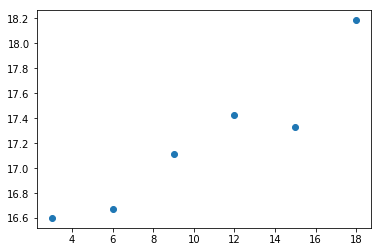
\includegraphics[width = 15cm]{n_currencies_dependence.png}
\caption{time dependence on number of currencies}
\label{fig:n_currencies_dependence}
\end{figure} 

Итого временные зависимости именно такие, какие и должны быть. Более подробно об этом можно посмотреть в тетрадке time measurement

\section{Тесты на реальных данных}
Исходное предположение - о линейной рекурентной зависимости в латентном пространстве, которое связано с исходным линейным преобразованием может быть и плохо применимо к реальным данным. Вообще говоря у нас так и получилось. Пример предсказания для реальных данных приведен на рисунке (\ref{fig:predictions_on_real})

\begin{figure}[!htb]
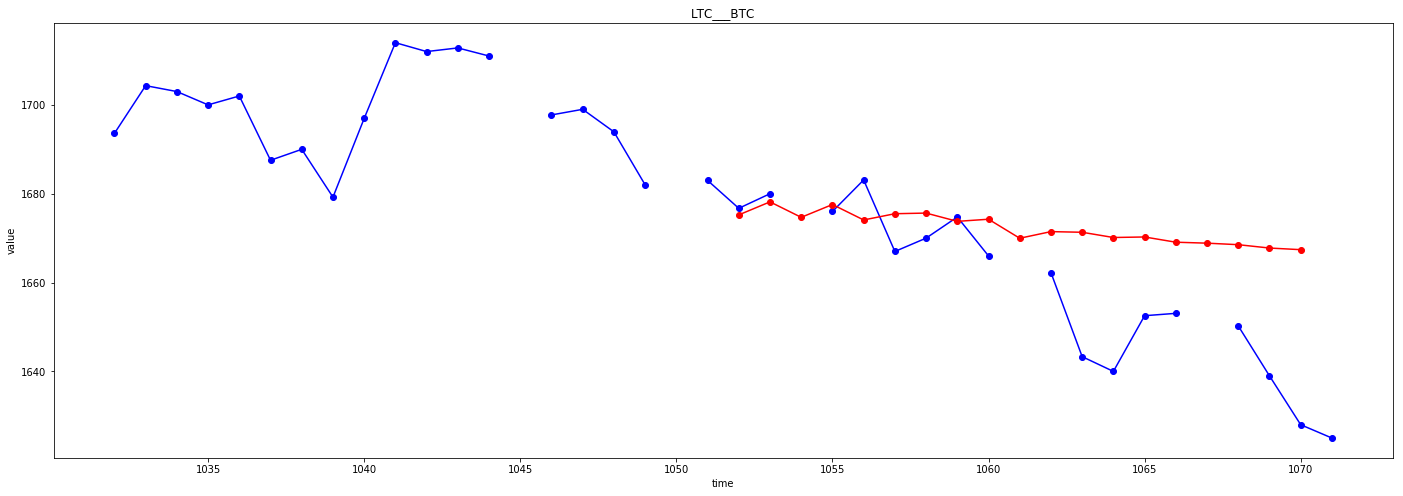
\includegraphics[width = 15cm]{predictions_on_real.png}
\caption{predictions for hitbtc data}
\label{fig:predictions_on_real}
\end{figure} 

В общем-то он апроксимирует прямой с небольшими, сходящими на нет отклонениями - причина такого поведения в общем-то уже была обговорена раньше - дело в том, для той рекурентной последовательности все собственные числа оказались по модулю меньше 1. Если бы хотя бы одна оказалась больше 1 то все совсем бы разошлось, а равенство модуля какой-то одной из них в точности единице это невероятная случаяность. В общем-то, к сожалению, это сильно ограничивает дальность прогноза.

Далее для всех датасетов мы зафитили нашу бибилотеку с размерностью латентного пространства равным 2, и изобразили на двухмерном графике точки, соответствующие исходным валютным парам. Эти графики можно посмотреть в тетрадках clustering и clustering other parameters. Для некоторых датасетов на этих графиках видна некая кластерная структура, для других нет.



\end{document}
